\documentclass[a4paper,12pt,liststotocnumbered]{scrartcl}

\usepackage[utf8x]{inputenc}
\usepackage{ngerman}
\usepackage{tabularx}
\usepackage{graphicx}
\usepackage{hyperref}
\usepackage{calc}
\usepackage{scrpage2}

\pagestyle{scrheadings}

\hypersetup{colorlinks=false,pdfborder=0 0 0}

% command for version
\newcommand{\lxVersion}[0]{1.0}

\chead[]{}
\lohead[Webtechnologie I - T09]{Webtechnologie I - T09}
\rohead[\today, Version: \lxVersion]{\today, Version: \lxVersion}

%\chead[{
%\lohead[Gateway- / Proxyserver]{Gateway- / Proxyserver}
%\rohead[Projektname: ProximusPrime]{Projektname: ProximusPrime}
%}]

\title{Anforderungsdokument Fotoalbum}
\author{Sebastian Eberlein, Sven Salzwedel - Team 09}

\begin{document}

\begin{figure}[h]
	\begin{center}
		
\includegraphics[width=\textwidth/2]{logo}
	\end{center}
\end{figure}

\begin{tabularx}{\textwidth}{lX}
	Fach:&Webtechnologie I\\
	Semester:&Sommersemester 2007\\
	Prüfungsleistung:&Praktischer Leistungsnachweis\\
	&\\
	Teammitglieder:&Sebastian Eberlein\\
	&Sven Salzwedel\\
	Teamnummer:&T09\\
\end{tabularx}

\begin{center}
\end{center}

\begin{center}
	\Large{\textbf{Thema:} Webbasiertes Fotoalbum}\\
\end{center}
\begin{center}
	\Large{\textbf{Anforderungsdokument}}\\
\end{center}

\begin{center}
	Datum: \today\\
	Version: \lxVersion
\end{center}

\newpage

\section*{Änderungshistorie}
\begin{description}
	\item[11. Mai 2007] Version 0.5, Erste Version zur Vorlage
		fertiggestellt (Eberlein, Salzwedel)
	\item[19. Mai 2007] Version 0.6, Überarbeitung laut Absprache, Punkt
		1.7 eingefügt, Projektplan, externe Komponenten angepasst
		(Eberlein, Salzwedel)
	\item[] Version 1.0, Angabe von Anforderungen an das
		Serverprogramm, Korrekturen, Angabe der Quellen (Eberlein,
		Salzwedel)
\end{description}
\newpage

%\maketitle
\tableofcontents

\newpage

\section{Einführung}
\subsection{Ziel}

Entwicklung einer webbasierten Benutzeroberfläche zur Darstellung von Fotos
welche zu Alben zusammengefasst werden können. Die Fotos und Alben sollen
dabei über eine ebenfalls webbasierte Administrationsoberfläche verwaltet
werden können.

\subsection{Überblick}

Das System besteht aus einer Client-Server Architektur, welche über HTTP
miteinander kommuniziert. Als Client zeigt ein Webbrowser (z.B. Mozilla
Firefox) die vom Server in HTML Dateien bereitgestellten Fotoalben dar. In der
Oberfläche können zusätzlich zu den Fotos auch Metadaten wie EXIF/IPTC sowie
die Kategorisierung mittels so genannter Tags angezeigt werden. Die Verwaltung
dieser Oberfläche geschieht über eine weitere Administrationsoberfläche,
welche über den gleichen HTTP Server ausgeliefert wird. Diese ist allerdings
nur einem Administrator zugänglich. Die nachfolgende Abbildung stellt die
Verbindung der Benutzer mit dem System schematisch dar.

\begin{figure}[bh]
	\begin{center}
		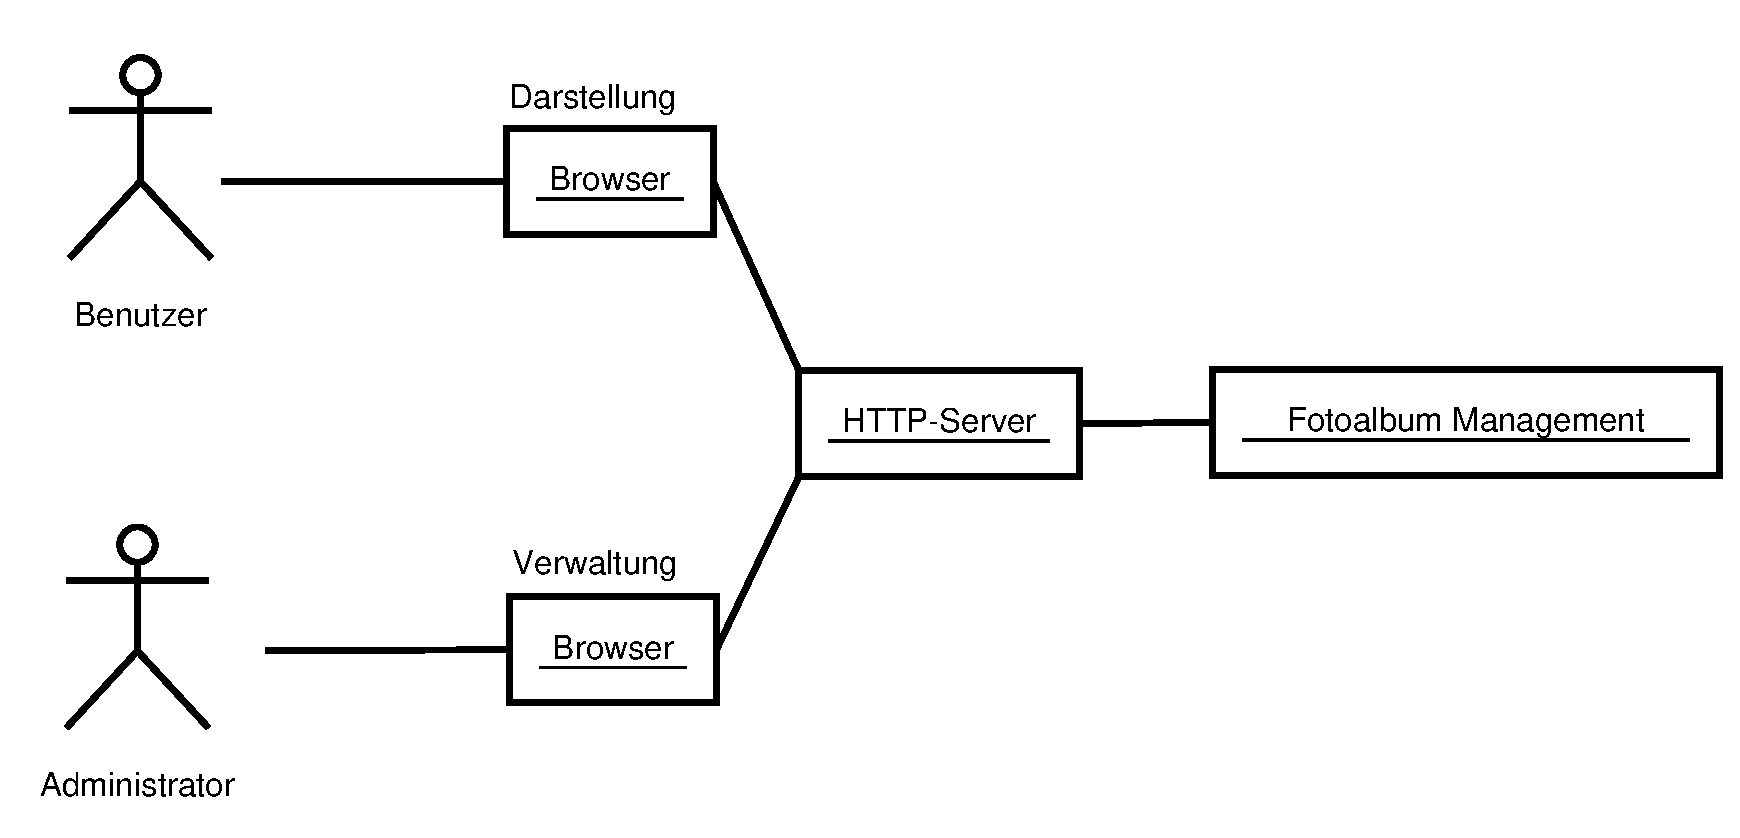
\includegraphics[width=\textwidth*3/4]{ueberblick}
		\caption{Kommunikationswege des Systems}
		\label{overview}
	\end{center}
\end{figure}

\newpage

Als Beispiel für die Darstellung eines solchen Fotoalbums dient das
nachfolgende Bildschirmfoto.

\begin{figure}[bh]
	\begin{center}
		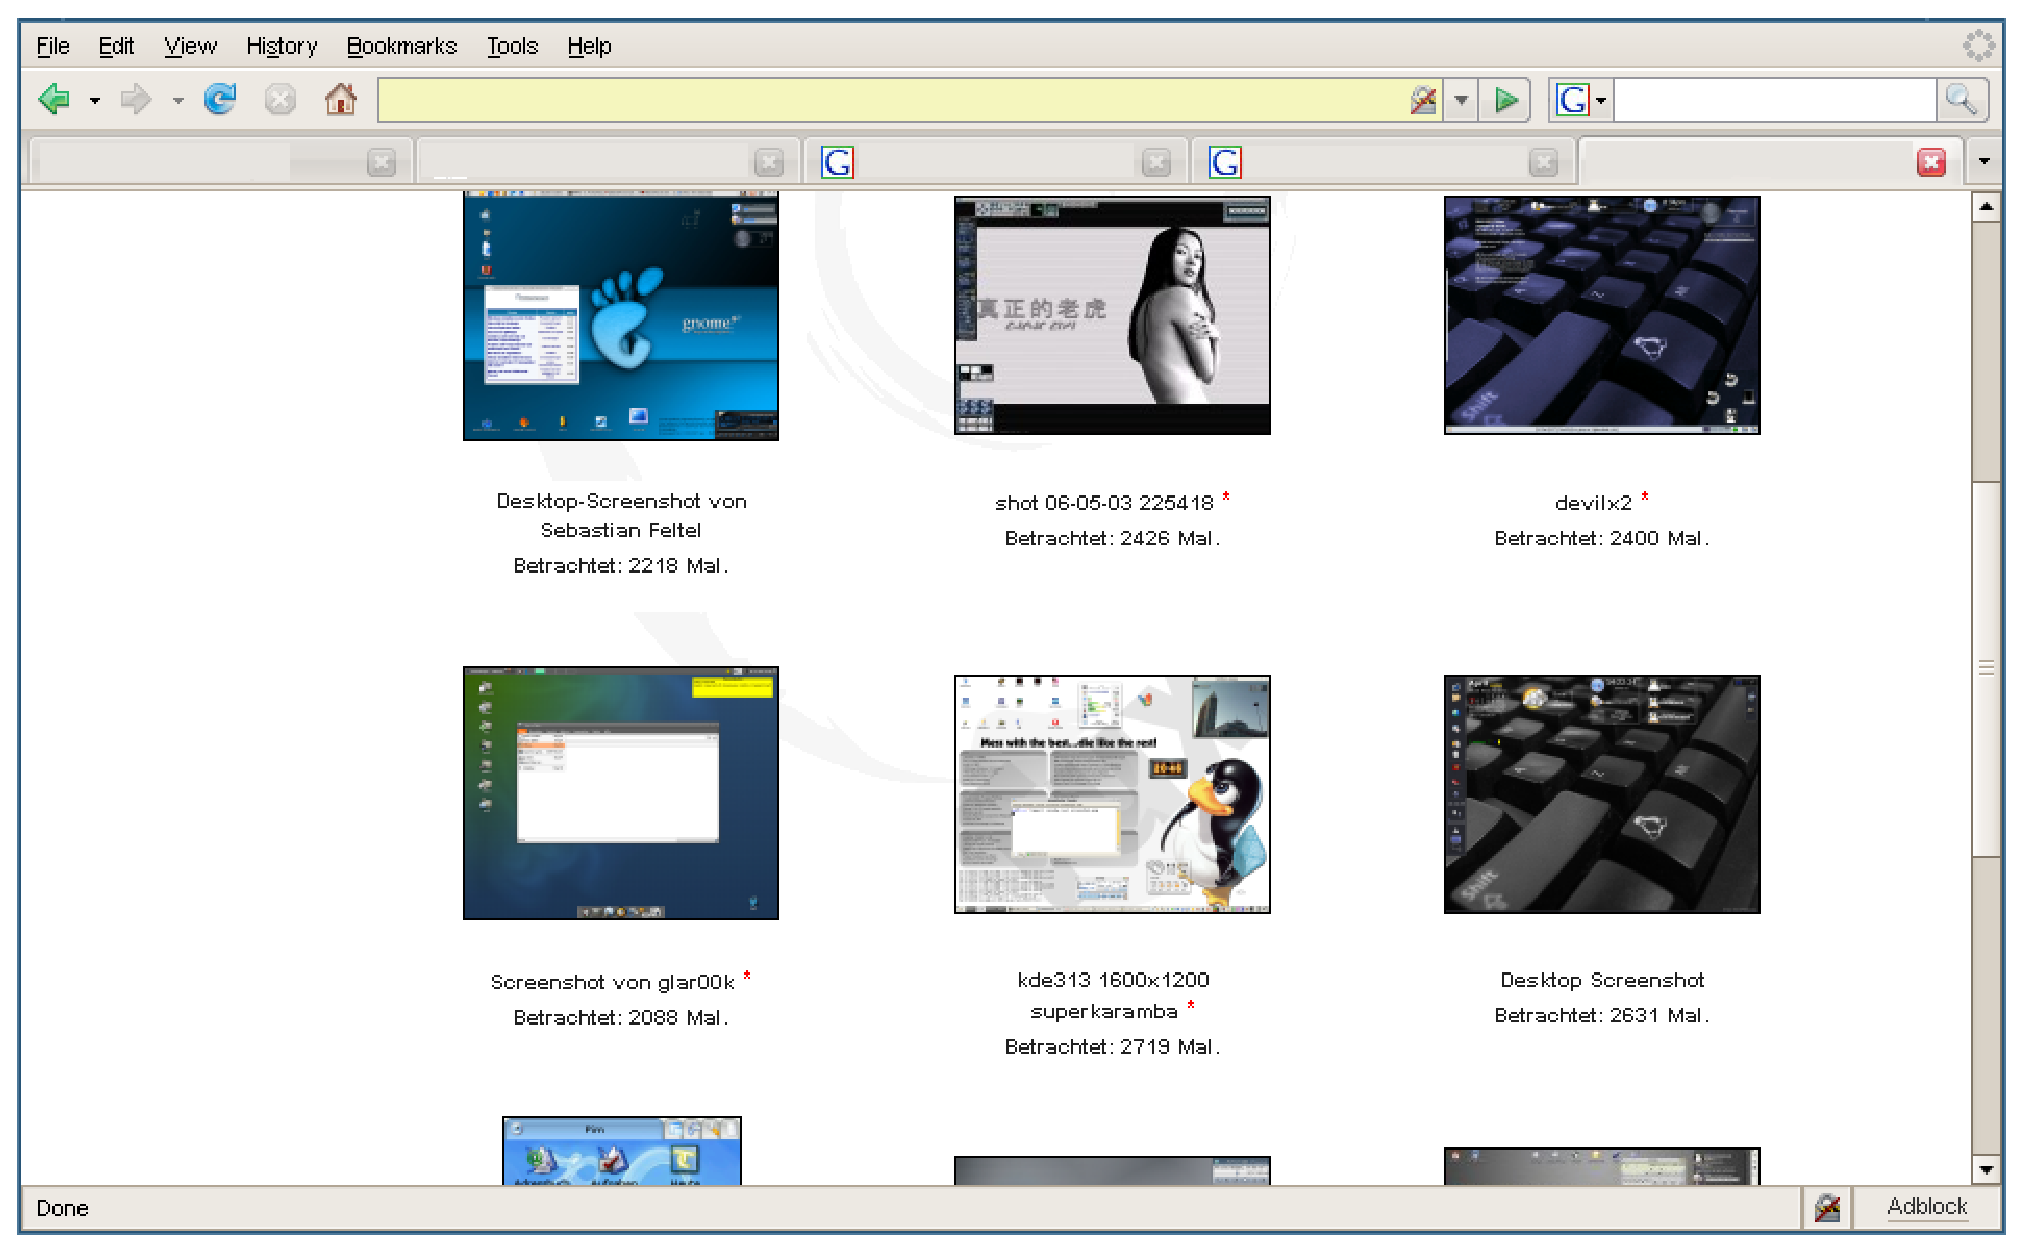
\includegraphics[width=\textwidth]{gallery}
		\caption{Beispiel für ein Fotoalbum}
		\label{sample}
	\end{center}
\end{figure}

\subsection{Definitionen, Akronyme und Abkürzungen}

%\begin{description}
%	\item[HTTP:]
%		\textbf{H}yper\textbf{T}ext \textbf{T}ransfer \textbf{P}rotocol
%	\item[HTML:]
%		\textbf{H}yper\textbf{T}ext \textbf{M}arkup \textbf{L}anguage
%	\item[XSLT:]
%		\textbf{E}xtensible \textbf{S}tylesheet \textbf{L}anguage
%		\textbf{T}ransformations
%	\item[EXIF:]
%		\textbf{E}xchangeable \textbf{I}mage \textbf{F}ile
%		\textbf{F}ormat, dient zur Speicherung von Textdaten in
%		Bilddateien
%	\item[IPTC:]
%		Genauer der IPTC-NAA-Standard, dient zur Speicherung von
%		Textdaten in Bilddateien
%	\item[AJAX:]
%		\textbf{A}synchronous \textbf{J}avascript \textbf{A}nd
%		\textbf{X}ML
%	\item[Metadaten:]
%		Albumtitel, Bildbeschreibung, EXIF und IPTC Daten,
%		Kommentare
%\end{description}

\begin{tabularx}{\textwidth}{|l|X|}
	\hline

	HTTP&\textbf{H}yper\textbf{T}ext \textbf{T}ransfer \textbf{P}rotocol\\

	\hline

	HTML&\textbf{H}yper\textbf{T}ext \textbf{M}arkup \textbf{L}anguage\\

	\hline

	XSLT&\textbf{E}xtensible \textbf{S}tylesheet \textbf{L}anguage
	\textbf{T}ransformations\\

	\hline

	EXIF&\textbf{E}xchangeable \textbf{I}mage \textbf{F}ile
	\textbf{F}ormat, dient zur Speicherung von Textdaten in Fotodateien\\

	\hline

	IPTC&Genauer der IPTC-NAA-Standard, dient zur Speicherung von
	Textdaten in Fotodateien\\

	\hline

	AJAX&\textbf{A}synchronous \textbf{J}avascript \textbf{A}nd
	\textbf{X}ML\\

	\hline

	SSL&\textbf{S}ecure \textbf{S}ocket \textbf{L}ayer\\
	\hline

	Metadaten&Albumtitel, Fotobeschreibung, EXIF und IPTC Daten,
	Kommentare\\

	\hline

	Album&Sammlung von Fotos die meist zeitlich in einem Kontext
	zueinander stehen (z.B. Weihnachtsfeier 2006)\\

	\hline

	Tag&Ein Tag ist ein frei bestimmbarer Name für eine Kategorie (z.B.
	Urlaub, Natur, Familienfeier)\\

	\hline

	taggen&zuordnen eines Fotos zu einem Tag\\

	\hline
\end{tabularx}

\newpage

\subsection{Beteiligte}

\begin{description}
	\item[Kontext] Praktischer Leistungsnachweis im Fach Webtechnologie I
		im Sommersemester 2007 an der FH Coburg
	\item[Auftraggeber] Prof. Dr. Wissmann, Dozent an der FH Coburg
	\item[Auftragnehmer] Sebastian Eberlein (6. Semester Informatik), Sven
		Salzwedel (6. Semester Informatik)
\end{description}

\subsection{Randbedingungen und Vorgaben}

Als Betriebssystem für den Server werden GNU/Linux (Debian 4.0) und Windows XP
vorrausgesetzt und sind Bedingung für zuverlässige Funktion. Auf dem System
muss Java in Version 1.5 oder höher intalliert sein. Als Client sind der
Internet Explorer in mindestens Version 6.0 oder der Mozilla Firefox in
Version 1.5 Vorraussetzung und wurden auf Funktionalität getestet. Als weitere
Vorraussetzungen sind die Angaben im Dokument \textit{PLN-Themen Überblick}
vom 03.05.2007 Punkt \textit{09. Fotoalbum} zu sehen.

\subsection{Abhängigkeiten}

Folgende Bibliotheken sind externe Komponenten und werden in das Projekt
integriert.

\begin{itemize}
	\item IPTC/EXIF Bibliothek
	\item Apache Derby Datenbank
\end{itemize}

\subsection{Lieferungen und Leistungen}

Ausgeliefert wird ein Archiv im ZIP-Format auf CD-ROM welches folgende
Komponenten enthält.

\begin{itemize}

	\item \textit{Dokumentation} Die Dokumentation besteht aus einem
		Installationsdokument, einer Generieranleitung, einem
		Spezifikationsdokument und einem Benutzerhandbuch

	\item \textit{Server} Der Server wird als Jar Datei lauffähig
		ausgeliefert.
	
	\item \textit{Installationsdateien} Dateien die für die Installation
		des Servers notwendig sind.

	\item \textit{Quellcode} Die Source-Dateien werden zusätzlich in einem
		ZIP-Archiv beigelegt.

\end{itemize}

\section{Architektur}
\subsection{Grobarchitektur}

Der Fotoalbumserver ist grob in 8 Komponenten, unterteilt die in verschiedenen
Farben in nachfolgendem Diagramm dargestellt werden. Der HTTP Server nimmt die
Anfragen der Clients entgegen und leitet sie, falls Korrektheit besteht, an
den Dispatcher weiter, sonst gibt er eine Fehlermeldung aus. Je nach Anfrage
wählt der Dispatcher das geeignete Modul für die Bearbeitung aus. Diese
Arbeitsmodule arbeiten mit der Datenbank und dem Dateisystem.  Sobald die
Anfrage bearbeitet wurde, wird mittels des HTML Responder die passende HTML
Seite zurück geliefert.

\begin{figure}[h]
	\begin{center}
		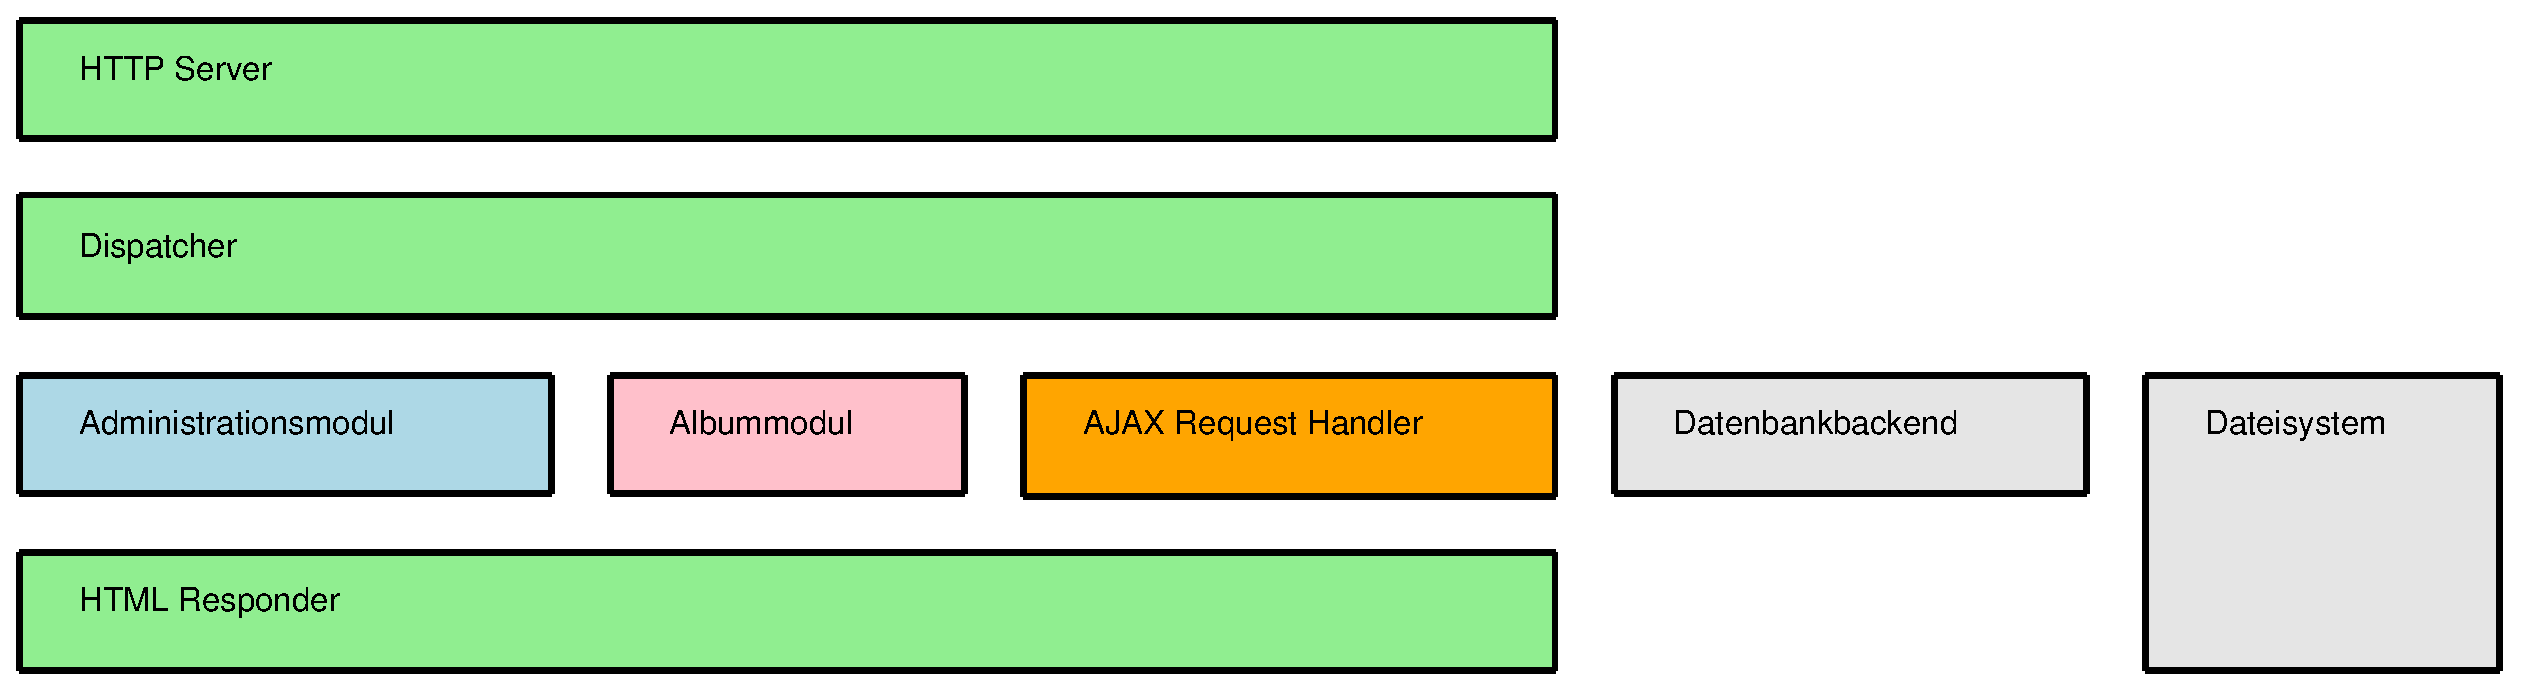
\includegraphics[width=\textwidth]{grobarchitektur}
		\caption{Aufbau des Fotoalbum Servers}
		\label{grobarchitektur}
	\end{center}
\end{figure}

\subsection{Detailarchitektur}

\subsubsection{HTTP Server}

Der HTTP Server wartet auf Verbindungen der Clients und arbeitet diese in
mehreren Threads ab. Dazu werden die HTTP Requests von einem HTTP Parser
geparst und auf Gültigkeit überprüft. Wenn der Request gültig ist, wird er an
den Dispatcher weiter geleitet. Ist der Request ungültig, wird ein HTTP Fehler
zurück gegeben. Der Server hält die Verbindung mit dem Client so lange offen,
bis der entsprechende HTTP Header zum Schließen der Verbindung mitgesendet
wird (HTTP 1.1). Der Server lässt mit SSL verschlüsselte HTTP Verbindungen zu.
Für die Administration der Fotoalben ist diese Art der Verbindung zwingend.

\subsubsection{Dispatcher}

Der Dispatcher untersucht den Request und ruft je nach Request URL das
passende Modul für die Verarbeitung des Request auf und liefert die benötigten
Daten aus dem Request.

\subsubsection{Administrationsmodul}

Wie bereits erwähnt ist dieses Modul nur über eine verschlüsselte Verbindung
erreichbar. Es liefert die HTML Dateien der Administrationsoberfläche aus und
nimmt Formulareingaben und Fotouploads des Administrators, die über das
Administrationsinterface mittels HTTP POST gesendet werden, entgegen. Die
Fotos werden im Dateisystem abgelegt und die Metadaten in einer Datenbank.
Änderungen an den Metadaten und Fotos werden mittels eines XSLT Prozessors
in eine HTML Seite umgewandelt und für die Auslieferung an die Clients im
Dateisystem gespeichert. Dieses Modul handelt weiterhin die
Benutzerauthentifizierung und Sitzungsverwaltung mittels Cookies ab.

\subsubsection{Albummodul}

Dieses Modul liefert je nach Request URL die passende HTML Seite bzw. das
entsprechende Foto an den Client. Da die HTML Seiten durch das
Administrationsmodul generiert werden ist der Aufwand für dieses Modul gering.

\subsubsection{AJAX Request Handler}

Der AJAX Request Handler ist die Kommunikationsschicht für die per Javascript
vom Client dynamisch angeforderten Daten welche in XML verpackt übertragen
werden. Mögliche Daten sind Informationen über das aktuelle Album (nächste
Foto URL) oder das aktuelle Foto (EXIF/IPTC).

\subsubsection{Datenbank \& Dateisystem}

Die Datenbank nimmt die Metainformationen wie Albumzugehörigkeit, EXIF/IPTC
Daten, Fototitel, Albumtitel und Kommentare auf. Im Dateisystem werden die
Fotos und die generierten HTML Dateien gespeichert.

\subsubsection{HTML Responder}

Der HTML Responder generiert aus der HTML-Seite welche als Antwort gesendet
werden soll den dazugehörigen HTTP Response und setzt im Fehlerfall den
passenden Statuscode. Dieser Response wird vom Server als Antwort auf einen
Request an den Client gesendet.

\newpage
\section{Anforderungen}
\subsection{Use-Cases}

\begin{figure}[bh]
	\begin{center}
%		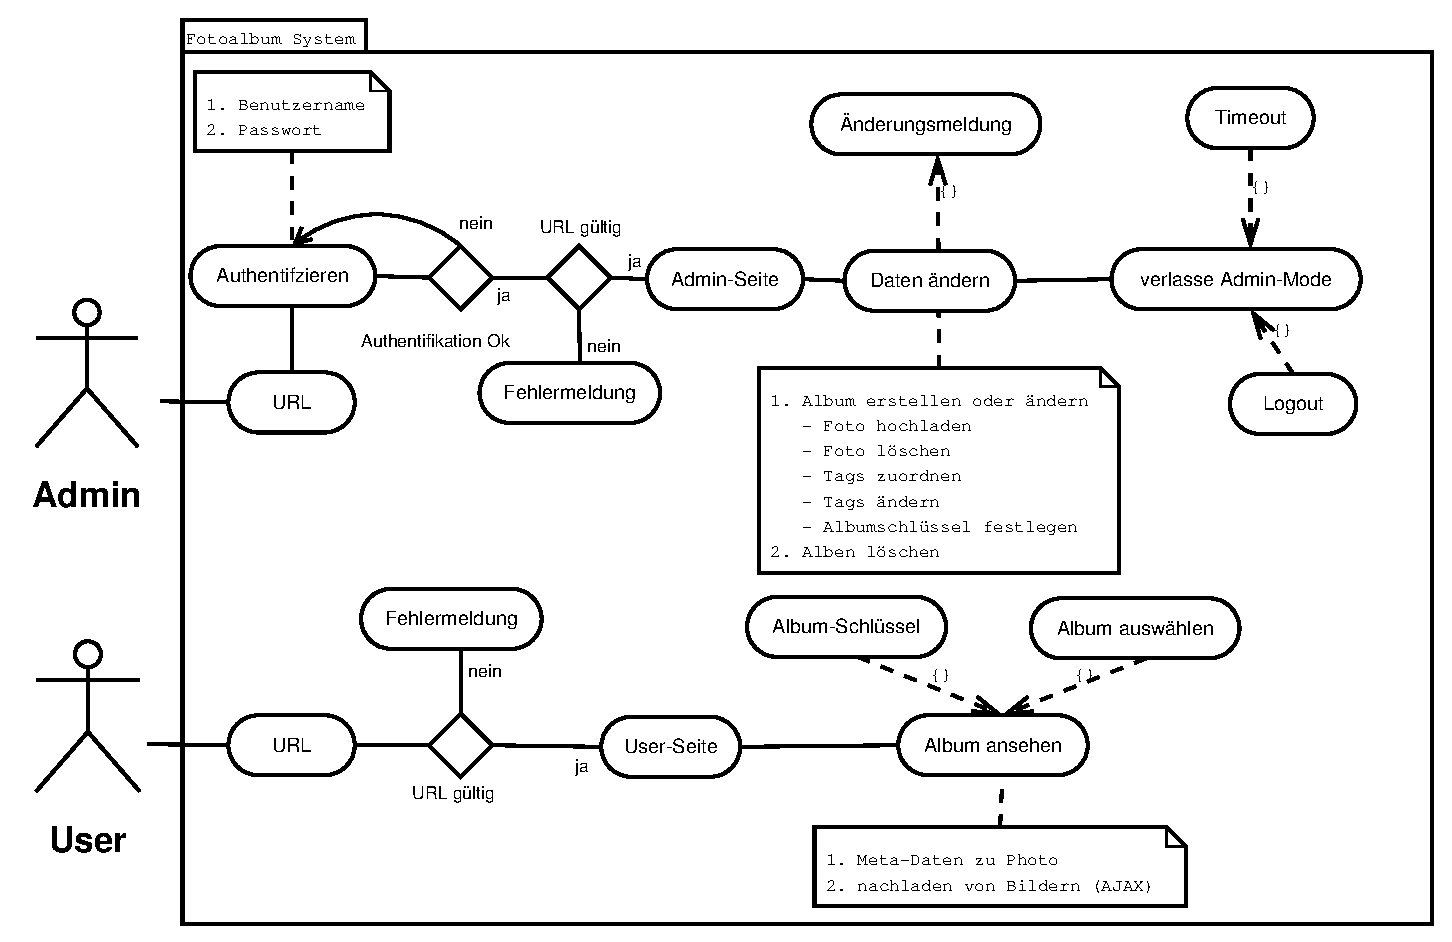
\includegraphics[angle=90,height=\textheight-6.4cm]{usecases}
		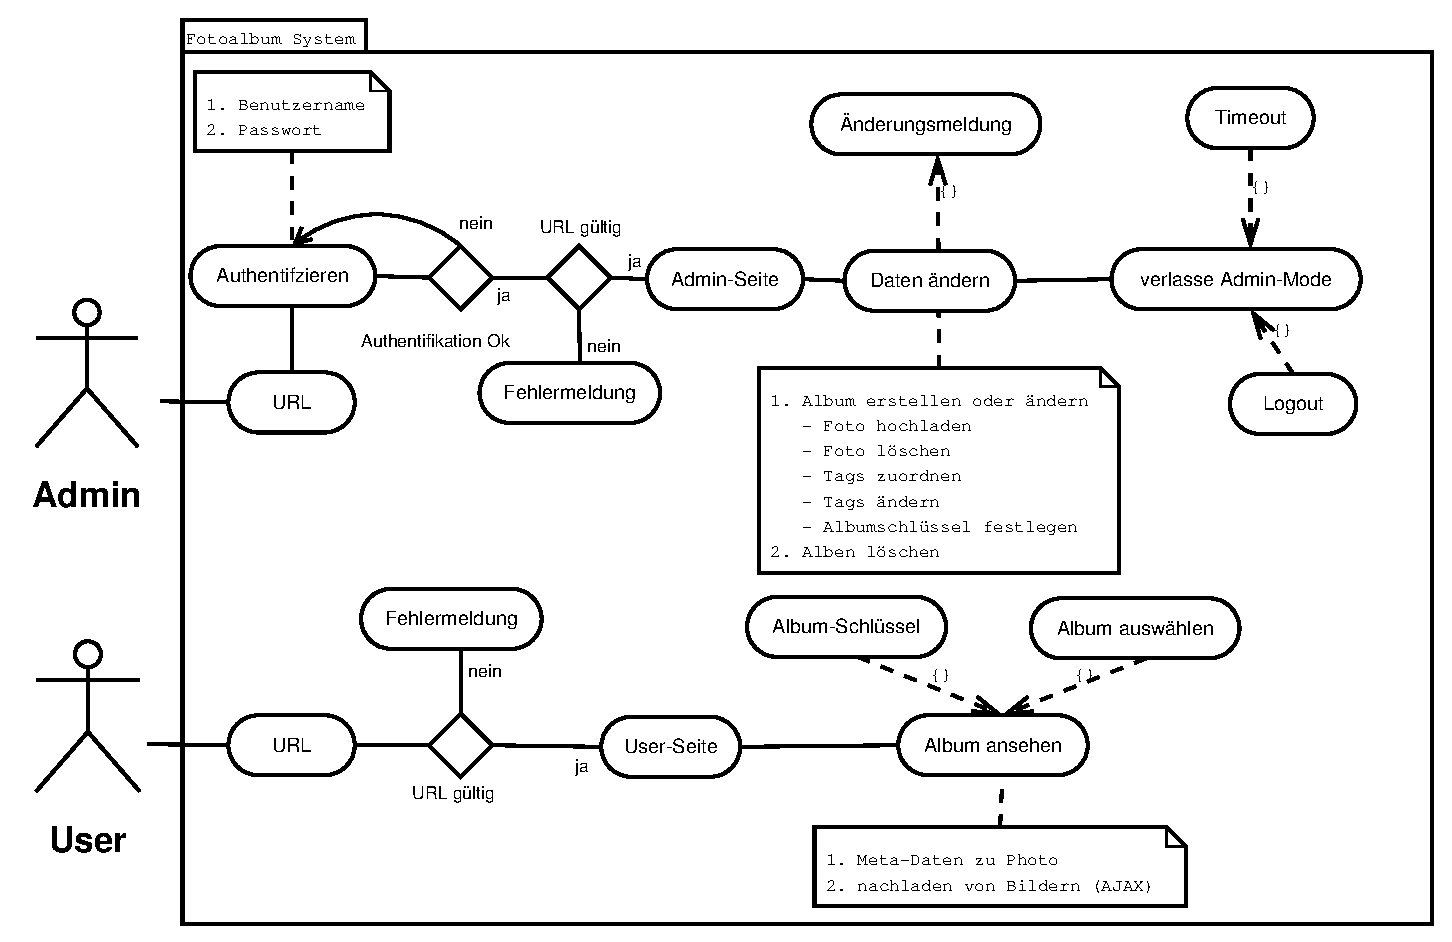
\includegraphics[width=\textwidth]{usecases}
		\caption{Use Cases}
		\label{usecases}
	\end{center}
\end{figure}

\newpage

\subsection{Funktionale Anforderungen}

\subsubsection{Anforderungen an die Oberfläche für den Benutzer}

\begin{itemize}
	\item Auflistung von Alben
	\item Anzeige von Fotos in einer Liste mit Miniaturansichten nach
		Auswahl eines Albums
	\item Anzeige eines Fotos in Detailansicht mit Fotobeschreibung nach
		Auswahl eines Fotos aus der Liste
	\item Auflistung von Fotos nach einem oder mehreren Tags
	\item Anzeige von EXIF/IPTC Daten zu einem Foto
	\item Anzeige von Fotos als Diashow
	\item Kommentierung von Fotos
\end{itemize}

\subsubsection{Anforderungen an die Oberfläche für den Administrator}

\begin{itemize}
	\item Administrator Authentifizierung
	\item Begrenzte Sitzungsdauer
	\item Nur eine Sitzung gleichzeitig möglich
	\item Erstellung von Alben
	\item Upload von Fotos und Zuordnung zu einem Album, sowie Speicherung
		im Dateisystem
	\item Angabe von Fotobeschreibungen
	\item Bearbeitung von Fotobeschreibungen
	\item Zuordnung von Fotos zu verschiedenen Tags
	\item Löschung von Fotos und Alben
	\item Löschung von Kommentaren
\end{itemize}

\subsubsection{Anforderung an das Serverprogramm}

\begin{itemize}
	\item Angabe des Pfades zur Speicherung von Fotos und der Ports  in
		einer Konfigurationsdatei
	\item Angabe des Administratorpassworts und -benutzernamen in einer
		Konfigurationsdatei
\end{itemize}

\subsection{Nichtfunktionale Anforderungen}

Es existieren keine Nichtfunktionalen Anforderungen.

\section{Priorisierung der Anforderungen}

\begin{enumerate}
	\item Angabe des Pfades zur Speicherung von Fotos und der Ports  in
		einer Konfigurationsdatei
	\item Auflistung von Alben
	\item Anzeige von Fotos in einer Liste mit Miniaturansichten nach
		Auswahl eines Albums
	\item Anzeige eines Fotos in Detailansicht mit Fotobeschreibung nach
		Auswahl eines Fotos aus der Liste
	\item Erstellung von Alben
	\item Upload von Fotos und Zuordnung zu einem Album, sowie Speicherung
		im Dateisystem
	\item Löschung von Fotos und Alben
	\item Angabe von Fotobeschreibungen
	\item Bearbeitung von Fotobeschreibungen
	\item Angabe des Administratorpassworts und -benutzernamen in einer
		Konfigurationsdatei
	\item Administrator Authentifizierung
	\item Begrenzte Sitzungsdauer
	\item Nur eine Sitzung gleichzeitig möglich
	\item Zuordnung von Fotos zu verschiedenen Tags
	\item Auflistung von Fotos nach einem oder mehreren Tags
	\item Anzeige von EXIF/IPTC Daten zu einem Foto
	\item Anzeige von Fotos als Diashow
	\item Kommentierung von Fotos
	\item Löschung von Kommentaren
\end{enumerate}

\section{Stufenplan}

\subsection{Stufe I}

In Stufe I wird der HTTP Server implementiert und erste
Darstellungsmöglichkeiten von Fotoalben. Die Funktionalität umfasst die Punkte
1 bis 9 aus der Prioritätsliste.

\subsection{Stufe II}

In Stufe II wird die Administrationsoberfläche mit SSL und Sitzungssteuerung
gesichert. Dies entpricht den Punkten 10 bis 13 aus der Prioritätsliste.

\subsection{Stufe III}

Die in Stufe III zu implementierenden Punkte 14 bis 16 umfassen die Metadaten
und das Tagging.

\subsection{Stufe IV}

Die Punkte 17 bis 19 werden in Stufe IV implementiert und umfassen ein
Template für eine Diashow und Kommentarfunktion für einzelne Fotos.

\section{Projektplan}

\subsection{Meilenstein MI (Stufen I \& II)}

\begin{tabularx}{\textwidth}{|l|X|X|}

	\hline

	\textbf{Datum}&\textbf{Tätigkeit}&\textbf{Bearbeiter}\\

	\hline

	19.05.2007&Erstellung des Anforderungsdokuments&Sebastian Eberlein \&
	Sven Salzwedel\\

	\hline 
	
	22.05.2007&Klassendiagramm&Sebastian Eberlein \& Sven Salzwedel\\

	\hline

	28.05.2007&Implementierung HTTP Server&Sven Salzwedel\\

	\hline

	28.05.2007&Implementierung Album Modul, Datenbankanbindung, Entwurf
	der HTML Templates&Sebastian Eberlein\\
	
	\hline

	04.06.2007&Implementierung Administrationsmodul&Sebastian Eberlein\\

	\hline

	04.06.2007&Administratorauthentifizierung \& Sitzungssteuerung&Sven
	Salzwedel\\

	\hline

\end{tabularx}

\subsection{Meilenstein MII (Stufe III)}

\begin{tabularx}{\textwidth}{|l|X|X|}

	\hline

	11.06.2007&EXIF/IPTC Unterstützung&Sebastian Eberlein\\

	\hline

	11.06.2007&Tagging Funktionalität&Sven Salzwedel\\

	\hline

\end{tabularx}

\subsection{Meilenstein MIII (Stufe IV)}

\begin{tabularx}{\textwidth}{|l|X|X|}

	\hline

	16.06.2007&Diashow Template&Sven Salzwedel\\

	\hline

	16.06.2007&Kommentarfunktion&Sebastian Eberlein\\
	
	\hline
	
\end{tabularx}

\subsection{Fertigstellung des Projekts}

\begin{tabularx}{\textwidth}{|l|X|X|}

	\hline

	22.06.2007&Test- und Integrationsphase&Sebastian Eberlein \& Sven
	Salzwedel\\

	\hline

	22.06.2007&Generierungsanleitung&Sebastian Eberlein\\

	\hline

	22.06.2007&Installationsanleitung \& Abgabe der Ergebnisse&Sven
	Salzwedel\\

	\hline

	25.06.2007&Präsentation&Sebastian Eberlein, Sven Salzwedel\\

	\hline

	parallel&Entwicklungsdokumentation \& Bedienungsanleitung&Sebastian
	Eberlein \& Sven Salzwedel\\

	\hline

\end{tabularx}

\end{document}
